%!TEX root = ../dissertation.tex

\hypertarget{(chap:capitolo2)}{}
\chapter{Processi e metodologie}
In questo capitolo verranno riportati in modo approfondito lo scopo e gli obiettivi dello stage, contestualizzazione delle attività alla realtà aziendale e scadenzario delle stesse.

\section{Contesto}
Il progetto generale nasce dalla visione di Filippo Sottovia, titolare dell'azienda, di realizzare un software decisionale di supporto che permettesse di soddisfare molteplici obiettivi quali:
\begin{itemize}
	\item agevolazione degli operatori nello svolgimento delle loro mansioni;
	\item facilitazione del processo decisionale richiedendo così lavoratori meno esperti;
	\item nascita nuove attività frutto del tempo risparmiato grazie all'aumento della produttività;
	\item condivisione in tempo reale delle informazioni sullo stato dei trasporti;
	\item stima di costi e profitti disponibile in ogni momento.
\end{itemize}

Il software fornisce un'interfaccia grafica web intuitiva che fa dell'usabilità la propria punta di diamante. Essa infatti persegue l'idea di rendere il più semplice possibile operare sul sistema senza però mancare di professionalità. Il sistema inoltre è equipaggiato con algoritmi che permettono di ottimizzare gli ordini organizzando al meglio le merci da trasportare ripartendole nei diversi camion della flotta, tenendo conto degli orari di carico e scarico, delle sedi dei clienti/fornitori, delle condizioni di traffico sulle strade, delle pause dovute per legge agli autisti e della particolarità delle merci.

\section{Introduzione al progetto}
L'azienda per permettere di stimare lo spazio occupato dalle merci ha sviluppato un'\glo{euristica}, questa riceve in input le merci da trasportare divise nei diversi ordini di consegna, le approssima a parallelepipedi e le dispone al meglio sul pianale del camion, sovrapponendole dove possibile, con l'obiettivo di ridurre al minimo lo spazio lineare occupato dalle stesse, così facendo si risparmia spazio per eventuali altre merci da caricare qualora arrivassero nuovi ordini.
A rendere ancora più complicato il lavoro dell'euristica riportiamo tre principali problemi da tenere in considerazione:
\begin{itemize}
	\item Stabilità degli oggetti: la faccia inferiore di ciascun oggetto deve poggiare per intero sulle facce superiori di altri oggetti sotto di sé o sul pianale del camion;
	\item Sequenza di scarico: ogni oggetto deve poter essere scaricato lateralmente o frontalmente, questo implica che non può avere intorno a sé merci che ne blocchino lo scarico, in quanto appartenenti ad ordini successivi;
	\item Baricentro degli oggetti: il peso delle merci deve essere equamente distribuito sul pianale del camion;
	\item Sovrapponibilità delle merci: alcune merci non sono sovrapponibili.
\end{itemize}

\section{Vincoli temporali, tecnologici e metodologici}
Nel periodo di stage svolto presso l'azienda mi è stato chiesto di tenere un \textit{diario} condiviso utilizzando \bit{DropBox}{dropbox}, nel suddetto mi si richiedeva di annotare giornalmente l'avanzare del lavoro riportando idee, osservazioni riguardanti criticità rilevate e positività riscontrate negli strumenti utilizzati. Nella cartella condivisa mi è stato chiesto di includere anche gli articoli accademici letti e le presentazioni fatte in azienda man mano che si proseguiva con lo stage.

La presentazione di metà stage è stata un evento importante al quale ha presenziato tutto il team di sviluppo, parte del personale d'amministrazione e il Professor De Giovanni che mi ha fornito preziosi consigli sugli obiettivi su cui orientare gli sforzi per la seconda metà dello stage alla luce di quanto ottenuto nella prima metà.

Prima di iniziare lo stage è stato concordato con l'azienda un piano di lavoro su un totale di 320 ore, lavorando 5 giorni a settimana, 8 ore per ciascun giorno. 

\section{Requisiti e obiettivi}
Nella tabella riportata di seguito vengono elencati gli obiettivi dello stage, a corredo degli stessi vi sarà un codice univoco ed una breve descrizione.

Ogni obiettivo è provvisto di un codice identificativo formato da una delle seguenti stringhe ob,de,op, che rappresentano il livello di importanza e da un numero incrementale positivo, che rispetta la seguente nomenclatura: 
\begin{figure}[htp]
	\centering
	[importanza][identificativo].
\end{figure}

Il livello di importanza di ciascun obiettivo può essere uno tra i seguenti:
\begin{itemize}
	\item Obbligatorio: individuato dalla stringa \textit{ob}, sono obiettivi fondamentali per la riuscita del progetto, il loro soddisfacimento dovrà verificarsi obbligatoriamente entro la fine dello stage, pena il fallimento dello stesso;
	\item Desiderabile: individuato dalla stringa \textit{de}, sono obiettivi secondari su cui però si nutre dell'interesse, il loro soddisfacimento è auspicabile entro la fine dello stage;
	\item Opzionale: individuato dalla stringa \textit{op}, sono obiettivi di contorno su cui si nutre poco interesse, la loro realizzazione si verificherà nel momento in cui si dovessero soddisfare tutti gli obiettivi obbligatori e desiderabili prima della fine dello stage.
\end{itemize}

Si prevede lo svolgimento dei seguenti obiettivi:
\begin{itemize}
	\item Obbligatori
	      \begin{itemize}
	      	\item \underline{\textit{ob01}}: individuazione e analisi \textit{constraints} modello 2D;
	      	\item \underline{\textit{ob02}}: modello matematico 2D con \textit{framework} di modellazione algebrica;
	      	\item \underline{\textit{ob03}}: traduzione modello in Python con l'ausilio di Google OR-Tools;
	      	\item \underline{\textit{ob04}}: test sul modello 2D e confronto con l'euristica;
	      	\item \underline{\textit{ob05}}: individuazione e analisi \textit{constraints} modello 2DR; 
	      	\item \underline{\textit{ob06}}: modello matematico 2DR con \textit{framework} di modellazione algebrica;
	      	\item \underline{\textit{ob07}}: traduzione modello in Python con l'ausilio di Google OR-Tools;
	      	\item \underline{\textit{ob08}}: test sul modello 2DR e confronto con l'euristica;
	      \end{itemize}
	\item Desiderabili
	      \begin{itemize}
	      	\item \underline{\textit{de01}}: individuazione e analisi \textit{constraints} modello 3D;
	      	\item \underline{\textit{de02}}: modello matematico 3D con \textit{framework} di modellazione algebrica;
	      	\item \underline{\textit{de03}}: traduzione modello in Python con l'ausilio di Google OR-Tools;
	      	\item \underline{\textit{de04}}: test sul modello 3D e confronto con l'euristica;
	      \end{itemize}
	\item Opzionali
	      \begin{itemize}
	      	\item \underline{\textit{op01}}: evoluzione euristica, fornita dall'azienda, con nuove funzionalità;
	      \end{itemize} 
\end{itemize}
\begin{figure}[H]
	\begin{center} 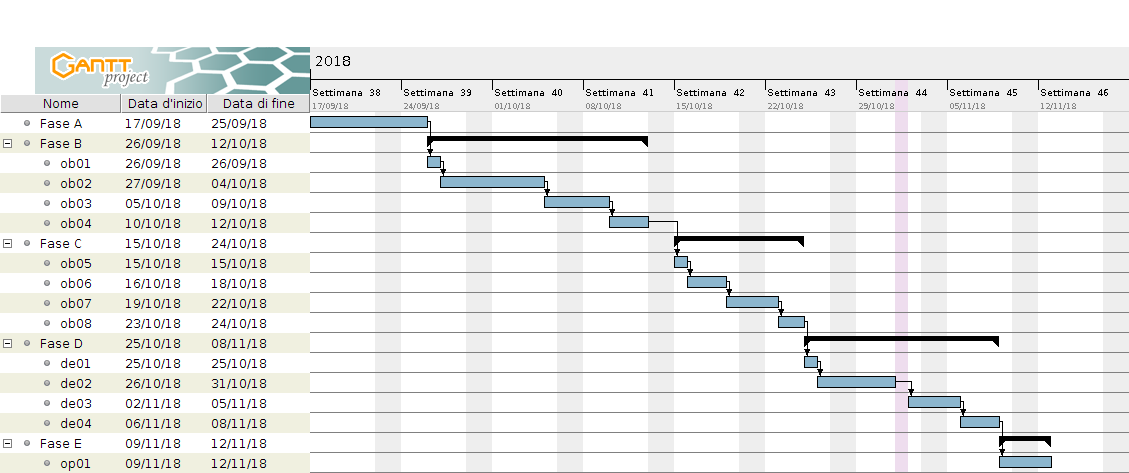
\includegraphics[scale=0.25]{figures/stage}
		\caption[Diagramma d Gantt]{Diagramma di Gantt dello stage.}
		\label{fig:gantt}
	\end{center}
\end{figure}
\section{Pianificazione}
Con le ore a disposizione per questo stage si è proceduto a organizzare come segue le attività:
\begin{itemize}
	\item \textbf{Formazione}: si è visto necessario approfondire la programmazione lineare e la letteratura correlata al problema del bin packing, imparare il linguaggio di programmazione \bit{Python}{python}, l'ambiente fornito dallo strumento \bit{Jupyter notebook}{jupyter} e imparare ad usare il framework \bit{Google Or-Tools}{ortools}.
	\item \textbf{Modello 2D}: questo periodo di stage ha richiesto la prototipazione, realizzazione e test del modello 2D e il confronto con l'euristica.
	\item \textbf{Modello 2DR}: questo periodo di stage ha richiesto la prototipazione, realizzazione e test del modello 2DR e il confronto con l'euristica.
	\item \textbf{Modello 3D}: questo periodo di stage ha richiesto la prototipazione, realizzazione e test del modello 3D e il confronto con l'euristica.
	\item \textbf{Lavoro sviluppo euristica}: periodo richiesto per realizzare delle funzionalità da integrare nell'euristica.
\end{itemize}

Ogni periodo di sviluppo di un modello sarà poi diviso a sua volta nelle seguenti attività:
\begin{itemize}
	\item analisi dei constraints
	\item prototipazione 
	\item test del modello
	\item confronto con l'euristica.
\end{itemize}

La pianificazione delle attività è stata distribuita come mostrato nella tabella~\eqref{tableofwork}.
\begin{center}
	\begin{tabular}{|l|l|c l|}
		\hline
		\multicolumn{2}{|l|}{\textbf{Durata in ore}}		&	\multicolumn{2}{l|}{\textbf{Descrizione dell'attività}}\\
		\hline
		\multicolumn{2}{|l|}{56}	&	\multicolumn{2}{l|}{\textbf{A}: Formazione}\\
		\hline
		\multirow{5}{1cm}{ } & 8  & \hspace{5mm}•\hspace{2mm} & Ricerca \textit{framework} di modellazione algebrica \\
		\multirow{5}{1cm}{ } & 24 & \hspace{5mm}•\hspace{2mm} & Studio di tale \textit{framework}                    \\
		\multirow{5}{1cm}{ } & 24 & \hspace{5mm}•\hspace{2mm} & Studio Google OR - Tools                             \\
		\hline
																											
		\multicolumn{2}{|l|}{104}	&	\multicolumn{2}{l|}{\textbf{B}: Versione modello 2D}\\
		\hline
		\multirow{5}{1cm}{ } & 8  & \hspace{5mm}•\hspace{2mm} & Individuazione ed analisi \textit{constraints}       \\
		\multirow{3}{1cm}{ } & 48 & \hspace{5mm}•\hspace{2mm} & Prototipazione modello                               \\
		\multirow{5}{1cm}{ } & 24 & \hspace{5mm}•\hspace{2mm} & Traduzione in Python - Google OR - Tools             \\
		\multirow{5}{1cm}{ } & 24 & \hspace{5mm}•\hspace{2mm} & Test e confronto con euristica                       \\	
		\hline
																											
		\multicolumn{2}{|l|}{72}	&	\multicolumn{2}{l|}{\textbf{C}: Versione modello 2D con rotazione}\\
		\hline
		\multirow{5}{1cm}{ } & 8  & \hspace{5mm}•\hspace{2mm} & Individuazione ed analisi \textit{constraints}       \\
		\multirow{3}{1cm}{ } & 24 & \hspace{5mm}•\hspace{2mm} & Prototipazione modello                               \\
		\multirow{5}{1cm}{ } & 16 & \hspace{5mm}•\hspace{2mm} & Traduzione in Python - Google OR - Tools             \\
		\multirow{5}{1cm}{ } & 16 & \hspace{5mm}•\hspace{2mm} & Test e confronto con euristica                       \\	
		\hline
																											
		\multicolumn{2}{|l|}{72}	&	\multicolumn{2}{l|}{\textbf{D}: Versione modello 3D con sovrapposizione}\\
		\hline
		\multirow{5}{1cm}{ } & 8  & \hspace{5mm}•\hspace{2mm} & Individuazione ed analisi \textit{constraints}       \\
		\multirow{3}{1cm}{ } & 32 & \hspace{5mm}•\hspace{2mm} & Prototipazione modello                               \\
		\multirow{5}{1cm}{ } & 16 & \hspace{5mm}•\hspace{2mm} & Traduzione in Python - Google OR - Tools             \\
		\multirow{5}{1cm}{ } & 24 & \hspace{5mm}•\hspace{2mm} & Test e confronto con euristica                       \\
		\hline
																													
		\multicolumn{2}{|l|}{16}	&	\multicolumn{2}{l|}{\textbf{E}: Lavoro sviluppo euristica}\\
		\hline
		\multirow{5}{1cm}{ } & 16 & \hspace{5mm}•\hspace{2mm} & Realizzazione nuove funzioni euristica               \\
		\hline
		\multicolumn{2}{|l|}{\textbf{Totale: 320}}		&	\multicolumn{2}{l|}{}\\
		\hline
																												
	\end{tabular}
	\captionof{table}{Pianificazione concordata nel piano di lavoro}
	\label{tableofwork}  
\end{center}
	
\section{Ambiente di lavoro}
\subsection{Metodi di sviluppo}
Il \glo{ciclo di vita} di un prodotto in Trans-Cel segue il \glo{modello incrementale}, formato da un periodo di concezione dell'idea, analisi della stessa, progettazione ed infine partendo dagli obiettivi più importanti si realizza il prodotto rilasciando periodicamente una versione dello stesso, questo dovrà mostrare le nuove funzionalità sviluppate dimostrando così l'incremento fatto. In quest'ottica lo sviluppo di un modello può essere associato ad un incremento, le cui \glo{milestone} è la ricezione dei risultati, a sua volta lo sviluppo di ciascun modello segue il modello incrementale, che può essere visto come l'insieme di tre principali attività:
\begin{itemize}
	\item Analisi letteratura: lettura articoli accademici riportanti modelli simili o idee per lo sviluppo degli stessi.
	\item Scrittura: scrittura del modello e integrazione con il sistema grazie al framework Or-Tools.
	\item Verifica: testing massivo e verifica delle soluzioni fornite.
\end{itemize}
Inoltre è possibile cogliere delle analogie con il modello di ciclo di vita \glo{agile} per quanto riguarda i \glo{brainstorming}, momenti di confronto creativo che stimolano il ragionamento in modo critico, utili per fare il punto della situazione oltre che esporre le problematicità che si stanno incontrando.

\subsection{Gestione di progetto}
Per quanto riguarda la gestione di progetto sono stati utilizzati alcuni strumenti descritti con maggiore dettaglio nel \hyperlink{(chap:capitolo6)}{\textbf{Capitolo 6}}. In generale per la gestione dei task da eseguire si è fatto uso di \bit{Taiga}{taiga}, uno strumento di \glo{project management}, per la gestione della comunicazione e condivisione informazioni si è fatto uso dell'applicazione \bit{Telegram}{telegram}, per la condivisione di documentazione e articoli si è fatto uso del servizio \bit{DropBox}{dropbox}, per il versionamento si è fatto uso del servizio \bit{GitHub}{github} per la familiarità dello strumento, infine per quanto riguarda l'interfaccia con cui versionare ho utilizzato \bit{git}{git} da terminale.
	
\subsection{Linguaggio di programmazione e ambiente di sviluppo}
Per la totalità dello stage si è lavorato utilizzando \bit{Jupyter notebook}{jupyter}. Con questo strumento è stato possibile scrivere programmi in linguaggio \bit{Python}{python} in modo molto agevole. 

Questo linguaggio di programmazione è orientato agli oggetti ed interpretato dinamicamente al momento dell'esecuzione da un interprete. \bit{Python}{python} risulta veramente versatile in quanto fornisce incredibili funzionalità utilizzabili in modo semplice e intuitivo, dispone di moltissimi moduli che permettono le più svariate operazioni, inoltre è stato possibile, grazie alla libreria \bit{Boost}{boost}, esporre costrutti \bit{C++}{cpp} a \bit{Python}{python} permettendo di utilizzarli nei propri programmi, questo ha permesso di mantenere efficienza e modularità.

\section{Analisi dei rischi}
In questa sezione vengono riportati i principali rischi che si prefiguravano all'inizio dello stage. Ciascuno di essi oltre ad avere una breve descrizione riporta il livello di rischio, in termini di pericolosità per la riuscita dello stage e come si possa fare per evitarlo:
\begin{itemize}
	\item \textbf{Difficoltà nelle tecnologie adottate}\\
	      Ad inizio stage è stato chiaro che \bit{Python}{python} avrebbe avuto un ruolo dominante nel progetto ma la mole di librerie ed estensioni rendeva il linguaggio troppo vasto da poter approfondire nella sua interezza, ed oltre a questo vi era il modulo Or-Tools e \bit{Pandas}{pandas} da approfondire e utilizzare.
	      \begin{itemize}
	      	\item \textbf{Livello di rischio}: Basso;
	      	\item \textbf{Contromisure}: Studiare approfonditamente il linguaggio \bit{Python}{python} e i moduli sopra citati.
	      \end{itemize}
	\item \textbf{Difficoltà di integrazione nel team}\\
	      Di fondamentale importanza per la riuscita di un progetto è la cooperazione con i colleghi e la creazione di un ambiente di lavoro sano e che stimoli la produttività, essendo un nuovo arrivato inserito in un ambiente soggetto a forte stress per le stringenti scadenze vi era la possibilità di entrare in conflitto con qualche collega.
	      \begin{itemize}
	      	\item \textbf{Livello di rischio}: Basso;
	      	\item \textbf{Contromisure}: Perseguire un atteggiamento positivo, critico e oggettivo.
	      \end{itemize}
	\item \textbf{Contrattempi dovuti a malattie e impegni}\\
	      Un rischio da tenere in considerazione è quello dovuto a impegni o malattie che precludano la possibilità di recarsi nel luogo di lavoro, data la durata dello stage è sicuramente possibile possa verificarsi.
	      \begin{itemize}
	      	\item \textbf{Livello di rischio}: Basso;
	      	\item \textbf{Contromisure}: Organizzare precedentemente ogni impegno non lavorativo e tempo di \glo{slack} per evitare contrattempi.
	      \end{itemize}
	\item \textbf{Difficoltà di stima dei tempi previsti}\\
	      Con un progetto di così lunga durata e l'inesperienza che ci portiamo appresso è possibile che vengano fatti degli errori di valutazione in termini di tempistiche per lo svolgimento delle diverse attività pianificate.
	      \begin{itemize}
	      	\item \textbf{Livello di rischio}: Medio;
	      	\item \textbf{Contromisure}: Rendere partecipi nella definizione del piano di lavoro persone esperte, come il tutor aziendale e il project manager.
	      \end{itemize}
\end{itemize}
